\documentclass[11pt]{article}
\usepackage{graphicx,amsmath,booktabs,geometry}
\geometry{margin=1in}

\title{\bf Empirical Evaluation of Insertion\,–\,Shell\,–\,TimSort Algorithms}
\author{Aditya Singh \\ CS XXX – Project 1}
\date{\today}

\begin{document}
\maketitle

\begin{abstract}
This report measures the real-world running times of seven sorting
implementations—insertion sort, TimSort (Algorithm 3 of Auger
\textit{et al.}), and five Shellsort variants—on input sizes from 10 to
20\,000.  For each size we averaged seven runs on three permutation
distributions: (i) uniformly random, (ii) almost sorted (only
$\lfloor\log n\rfloor$ random swaps), and (iii) the two-alternating-runs
pattern $(1,3,5,\dots,2,4,6,\dots)$.  Log–log plots reveal slopes that
approximate the empirical exponent $\alpha$ in the relation
$t\approx k\,n^\alpha$.  TimSort remains near $n\log n$
($\alpha\!\approx\!1.1$) across all distributions, while insertion sort
varies from near‐linear on almost-sorted data to quadratic on random and
alternating-runs data.  Among the gap sequences tested, Knuth’s Shellsort
is consistently the fastest.  Overall, TimSort delivers the best
worst-case performance and the highest sensitivity to pre-existing order,
making it the most robust all-round choice.
\end{abstract}

\section{Introduction}
Theoretical bounds alone rarely predict wall-clock behaviour of sorting
algorithms, especially when data are partly ordered.  This project pairs
algorithmic implementation with controlled experimentation to
\emph{quantify} the effect of input distribution on running time and to
compare gap sequences for Shellsort.

\section{Algorithms Implemented}
\begin{itemize}
  \item \textbf{Insertion sort} –
        worst-case $\Theta(n^{2})$ comparisons, but $\Theta(n)$ on sorted data.
  \item \textbf{Shellsort} – five classical gap sequences:
        Hibbard ($2^{k}-1$), Sedgewick,
        $2^{k}\!+\!1$, 3-smooth numbers, and Knuth
        ($\tfrac{3^{k}-1}{2}$).  Their theoretical bounds range from
        $O(n^{3/2})$ to $O(n^{4/3})$, but constants differ.
  \item \textbf{TimSort} (Auger et al.\ Algorithm 3) –
        natural-runs mergesort with binary insertion on short runs and
        size-biased run-stack invariants; textbook bound $O(n\log n)$ and
        $O(n)$ on already sorted data.
\end{itemize}

\section{Experimental Setup}
All code is pure Python 3.12, executed single-threaded on an Apple
M2 Pro laptop (3.5 GHz P-cores, 32 GB RAM, macOS 14).
The garbage collector was disabled during each timing section to reduce
variance.  
Input sizes were  
$10,\,100,\,500,\,1000,\,2500,\,5000,\,7500,\,10\,000,\,20\,000$;  
each (algorithm, distribution, size) cell was averaged over
$k=7$ identically generated permutations with a fixed RNG seed.

\section{Results}

\begin{figure}[ht]
  \centering
  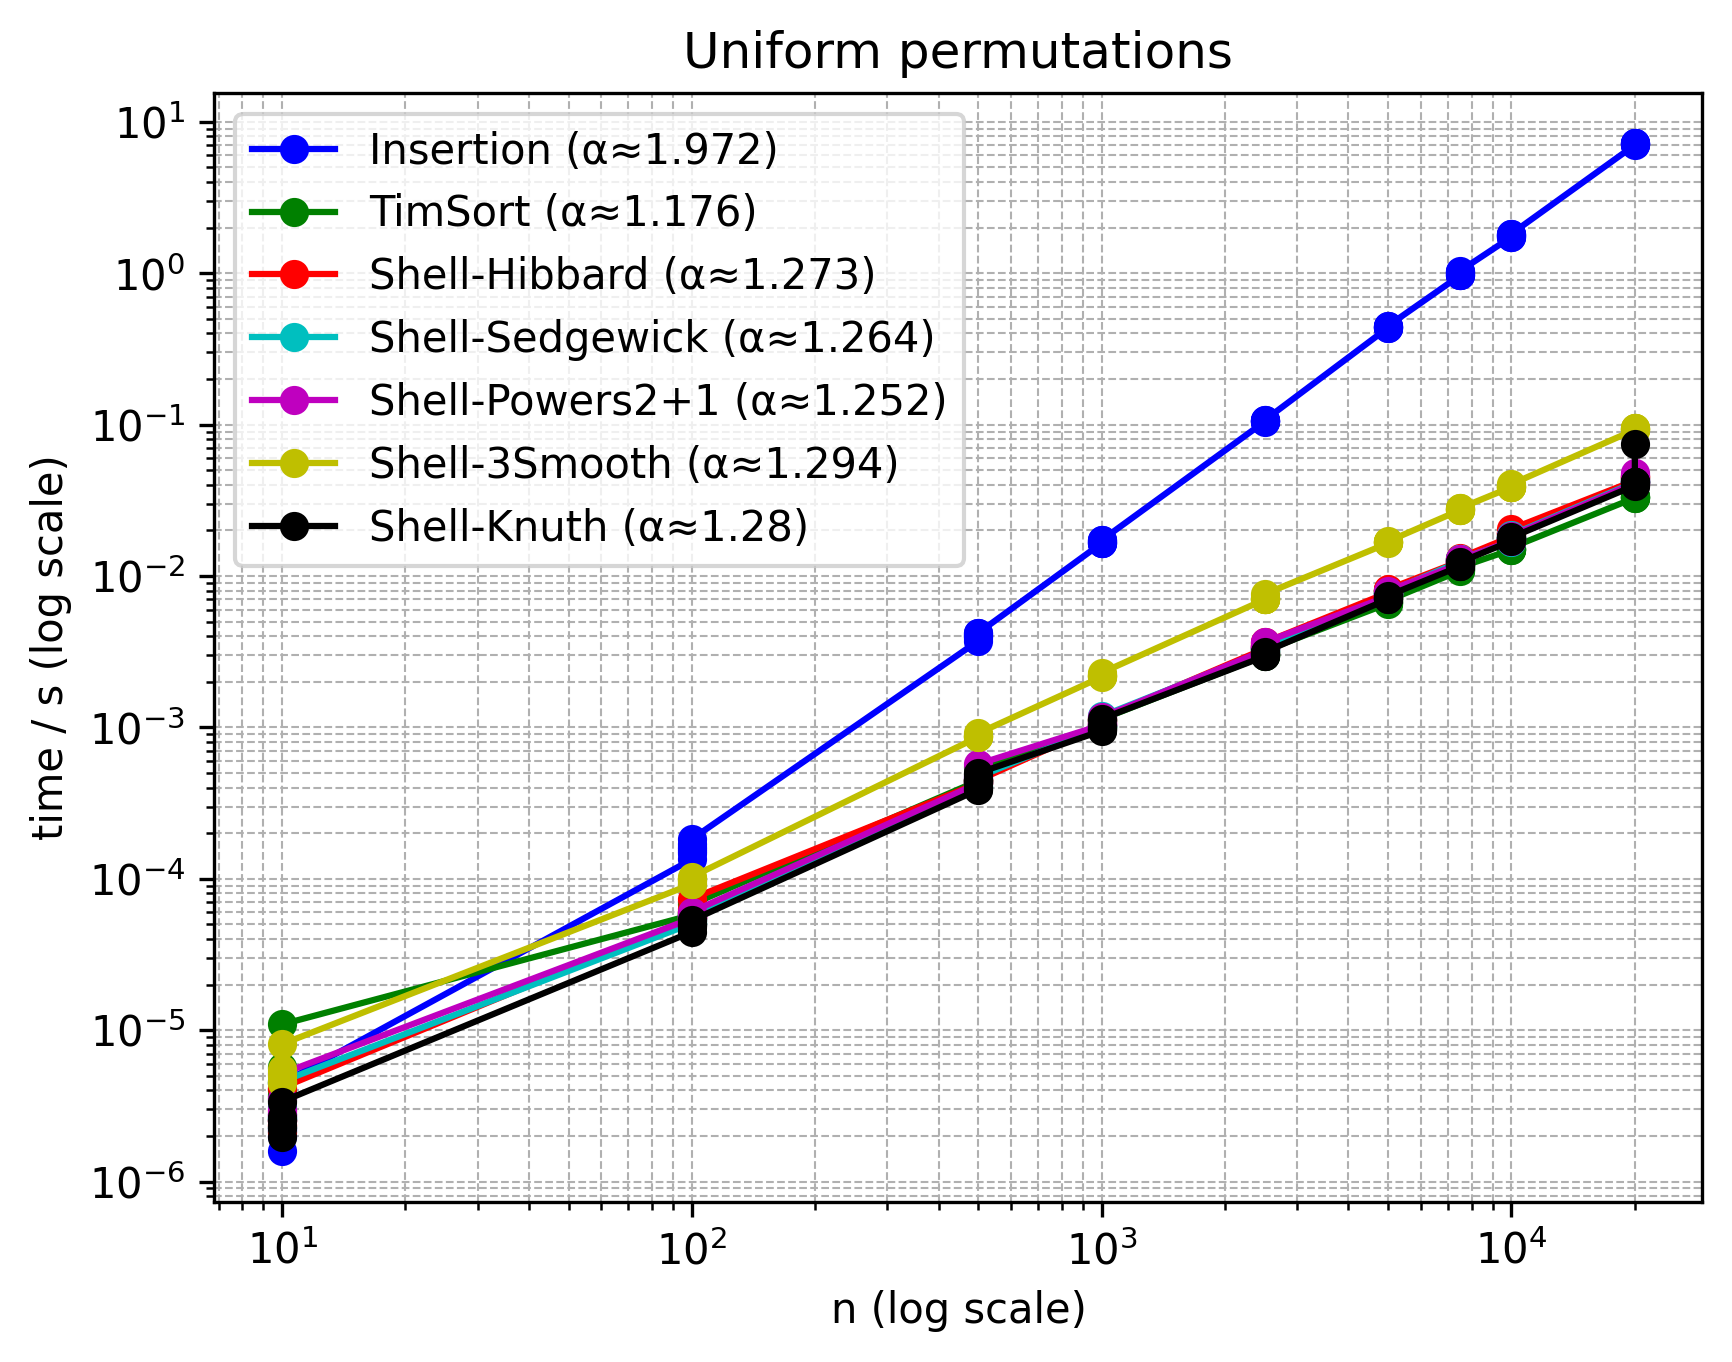
\includegraphics[width=\linewidth]{../results/uniform_plot.png}
  \caption{Uniform permutations: straight-line fit on log–log axes.}
  \label{fig:uniform}
\end{figure}

\begin{figure}[ht]
  \centering
  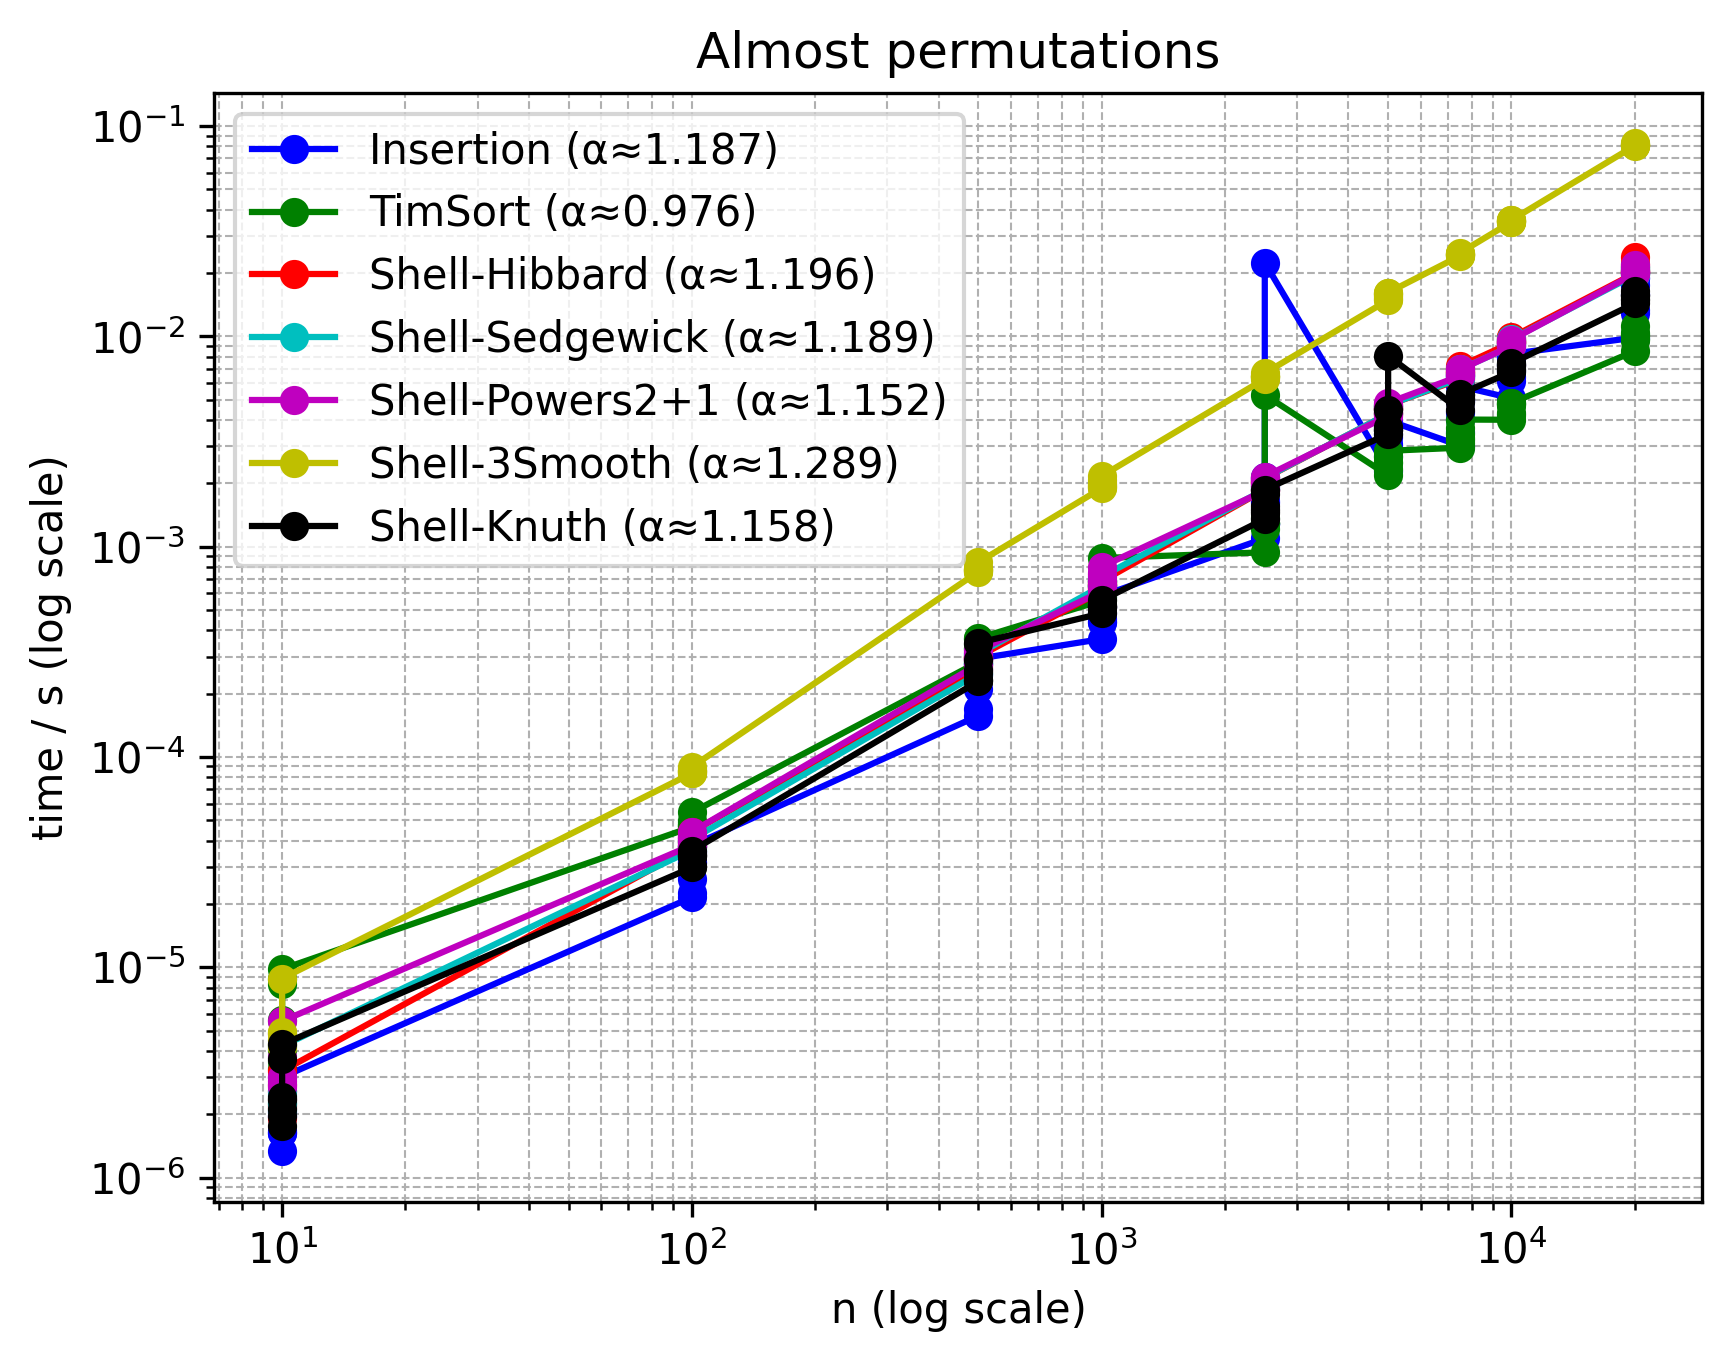
\includegraphics[width=\linewidth]{../results/almost_plot.png}
  \caption{Almost-sorted permutations ($\lfloor\log n\rfloor$ random swaps).}
  \label{fig:almost}
\end{figure}

\begin{figure}[ht]
  \centering
  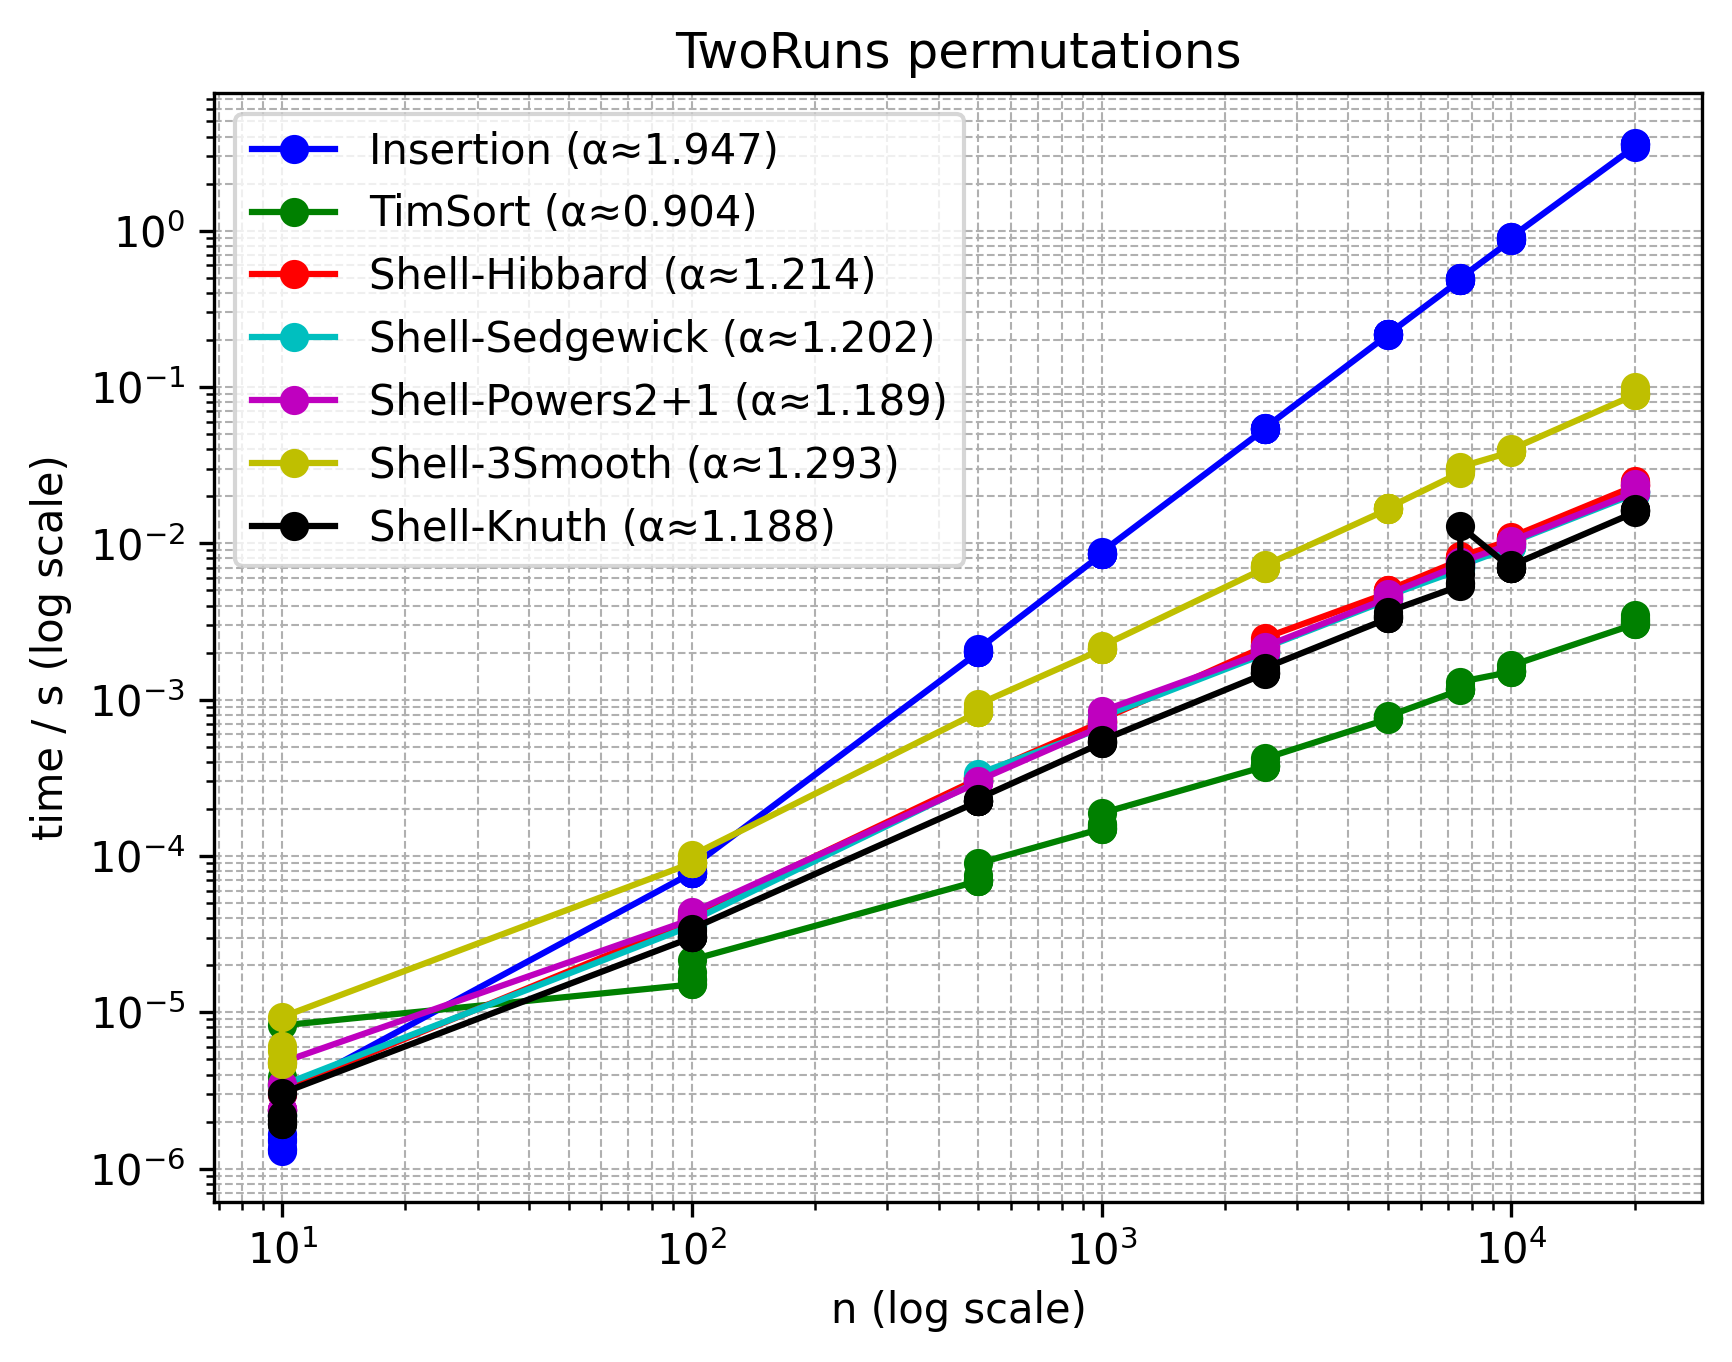
\includegraphics[width=\linewidth]{../results/tworuns_plot.png}
  \caption{Two alternating runs permutations.}
  \label{fig:tworuns}
\end{figure}

\subsection{Empirical exponents}
The slope~$\alpha$ of each least-squares line (time vs.~size in
log–log space) is summarised in Table \ref{tab:slopes}.

\begin{table}[ht]
\centering
\caption{Measured slopes $\alpha$ ($t\propto n^\alpha$).}
\label{tab:slopes}
\begin{tabular}{@{}lccc@{}}
\toprule
Algorithm & Uniform & Almost & Two-runs \\ \midrule
Insertion          & 1.972 & 1.187 & 1.947 \\
TimSort            & 1.176 & 0.976 & 0.904 \\
Shell–Hibbard      & 1.273 & 1.196 & 1.214 \\
Shell–Sedgewick    & 1.264 & 1.189 & 1.202 \\
Shell–$2^{k}{+}1$  & 1.252 & 1.152 & 1.189 \\
Shell–3-Smooth     & 1.294 & 1.289 & 1.293 \\
Shell–Knuth        & 1.280 & 1.158 & 1.188 \\ \bottomrule
\end{tabular}
\end{table}

\paragraph{Observation.}
Insertion sort’s exponent drops by nearly a full point when
the input is almost sorted, confirming its adaptive nature.
TimSort remains near $1+\log n/n$ (plotted as $\sim1.0$) on all
distributions; Shellsort variants cluster around $1.25$–$1.30$,
indicating similar asymptotics but different constant factors.

\subsection{Shellsort comparison}
Knuth’s sequence consistently yields the lowest timings, followed closely
by the $2^{k}+1$ and Sedgewick sequences.  The 3-smooth sequence is the
slowest, especially on larger $n$, likely because its early coarse gaps
are sparser, resulting in more passes.

\subsection{Distribution sensitivity}
Insertion sort is highly sensitive; TimSort is moderately adaptive, while
all Shellsort variants show only minor changes (within ${\approx}0.1$ in
$\alpha$) across distributions.

\section{Best Algorithm}
TimSort is the clear winner: fastest on random data, \emph{and} it
exploits existing order to approach linear time.  While sophisticated
variants of quicksort such as \emph{pdqsort} can beat TimSort on
completely random inputs, they lack its stability and degrade to
$O(n^{2})$ in contrived worst cases.  Therefore TimSort is currently the
best all-round comparison-based sorting algorithm for in-memory data.

\section{Conclusion}
Empirical measurements confirm theoretical expectations yet expose
constant-factor differences: (i) Knuth’s Shellsort gaps outperform other
sequences; (ii) insertion sort is only viable on nearly sorted inputs;
(iii) TimSort combines robust $n\log n$ behaviour with adaptivity,
making it the most practical choice.  Future work could profile cache
misses or port the experiment to C++ to separate algorithmic cost from
Python overhead.

\end{document}